\documentclass[sigplan,screen]{acmart}
\usepackage{graphicx}

%%
%% \BibTeX command to typeset BibTeX logo in the docs
\AtBeginDocument{%
  \providecommand\BibTeX{{%
    \normalfont B\kern-0.5em{\scshape i\kern-0.25em b}\kern-0.8em\TeX}}}

%% Rights management information.  This information is sent to you % when you
%complete the rights form.  These commands have SAMPLE % values in them; it is
%your responsibility as an author to replace % the commands and values with
%those provided to you when you % complete the rights form.
\setcopyright{acmcopyright}
\copyrightyear{2018}
\acmYear{2018} \acmDOI{10.1145/1122445.1122456}

%% These commands are for a PROCEEDINGS abstract or paper.
% \acmConference[Woodstock '18]{Woodstock '18: ACM Symposium on Neural Gaze
% Detection}{June 03--05, 2018}{Woodstock, NY} \acmBooktitle{Woodstock '18: ACM
% Symposium on Neural Gaze Detection, June 03--05, 2018, Woodstock, NY}
% \acmPrice{15.00} \acmISBN{978-1-4503-XXXX-X/18/06}

%%
%% Submission ID. % Use this when submitting an article to a sponsored event.
%You'll % receive a unique submission ID from the organizers % of the event, and
%this ID should be used as the parameter to this command.
%%\acmSubmissionID{123-A56-BU3}

%%
%% end of the preamble, start of the body of the document source.
\begin{document}
\title{Solving the Traveling Salesman Problem with Genetic Hill-Climbing}

%%
%% The "author" command and its associated commands are used to define % the
%authors and their affiliations. % Of note is the shared affiliation of the
%first two authors, and the % "authornote" and "authornotemark" commands % used
%to denote shared contribution to the research.
\author{Aaron Cummings}
\authornote{All authors contributed equally to this research.}
\email{acummi28@students.kennesaw.edu}
\orcid{0000-0001-5900-9841}
\affiliation{%
    \institution{College of Computing and Software Engineering }
    \streetaddress{1100 South Marietta}
    \city{Marietta}
    \state{Georgia}
    \country{USA}
    \postcode{30060}
}

\author{Andy Vu}
\authornotemark[1]
\email{avu5@students.kennesaw.edu}
\affiliation{%
    \institution{College of Computing and Software Engineering }
    \streetaddress{1100 South Marietta}
    \city{Marietta}
    \state{Georgia}
    \country{USA}
    \postcode{30060}
}

%%
%% By default, the full list of authors will be used in the page % headers.
%Often, this list is too long, and will overlap % other information printed in
%the page headers. This command allows % the author to define a more concise
%list % of authors' names for this purpose.
\renewcommand{\shortauthors}{Cummings et al.}

%%
%% The abstract is a short summary of the work to be presented in the % article.
\begin{abstract}

\end{abstract}

%%
%% Keywords. The author(s) should pick words that accurately describe % the work
%being presented. Separate the keywords with commas.
\keywords{Algorithms, Hill-Climbing, Traveling Salesman, Genetic Algorithms, NP-hard, Exaustive Search, Branch and Bound, Heuristic}

%%
%% This command processes the author and affiliation and title % information and
%builds the first part of the formatted document.
\maketitle

\section{Introduction}
The history of the traveling salesman problem is unclear, however since its
inception it has been a problem that has continued to puzzle mankind even until
this day. The problem builds from finding a Hamiltonian cycle which can be
defined as a path in an undirected graph where each vertex is visited exactly
once. The traveling salesman problem builds upon this by requiring every vertex
to be visited once except for the starting vertex where there must be a path
from the end vertex back to the beginning. Thus, the start vertex is visited
twice, once in the beginning and lastly once at the end. It further pushes the
complication of these tasks by now asking of the many possible paths that exist,
which path provides the shortest length of the circuit. This type of problem is
critical to not only salesman which the name of the problem comes from, but for
many modern-day operations and businesses ranging from delivery trucks to flight
paths for planes. There have been many attempts at solving the traveling
salesman ranging from exact solutions which only work for small problem sizes to
heuristic models that give approximations. Once the problem enlarges these
outdated exact solutions are not capable of producing an answer. Here is where
suboptimal heuristic algorithms come into play.  In this paper, we propose a
method to combine two individual heuristic algorithms, hill climbing and genetic
algorithm, to create a genetic hill climbing algorithm that generates an
approximate solution to the traveling salesman problem within a reasonable time.
The intuition for this approach is to combine the aspects of each individual
algorithm to complement their respective weaknesses.

\section{Problem Definition}
The traveling salesman problem is modelled as an undirected weighted graph where
the vertices represent cities while the graph’s edges represent the paths. The
distances of the paths are then represented as the weights of the edges. There
are no limitations in how the graph is designed other than the requirement that
there must be a Hamiltonian circuit that possesses an edge from the final vertex
back to the starting vertex. This is the crucial step that separates a
Hamiltonian circuit from the traveling salesman problem. Graphs that are
complete, meaning there are paths to every node from any single node provides a
larger complexity given that there are more paths and edge weights to consider.
This generates the maximum number of possible paths thus finding the shortest
provides a difficult task. Realistically this does not exist as it would be
nearly impossible to find a road from one city to another without passing
through another city or in this case a vertex or without backtracking and
visiting another city or vertex.

Symmetrical traveling salesman problems are situations in the graph design where
the distances between two cities are the same in each opposite direction. This
is well represented in a road path where the route from once city to another and
back is simply just the opposite way but same length. This is not to be confused
with a graph that is connected but not complete. It is still possible for the
traveling salesman problem to exist where there are cities without direct paths
to other cities that satisfies the condition of the problem. Asymmetrical graph
design can include paths that are different weights from one city to another in
comparison to the opposite direction. In addition to this, asymmetrical design
can also have scenarios where paths only exist in one direction which
essentially puts the weighted edge at a length of zero. Real world examples of this
may include one-way streets, or flight paths.

For our implementation purposes and the design our of solutions to the traveling
salesman problem we have designed a variety of graph environments that start at
a minimum with five vertices however, these graphs eventually scale to a maximum
of 500 vertices. Our created graph dataset uses an adjacency matrix as the data
structure to store the values of the graph where the edges are randomized with
an upper bound weight of 100. Instead of a complete graph our graph environment
uses a randomized pattern to delete nodes from a complete graph to create a
symmetrical graph with some edges missing. This can be showcased below in figure
\ref{fig:example_graph}. We have created a function that uses the
squared number of vertices multiplied by a constant of .22 to assign a value as
the number of deletions to occur within a specified graph. <INSERT REASON FOR
.22 CONSTANT VALUE>

Even though a complete graph causes difficulty in finding the most
optimal path due to the sheer number of possibilities, implementing a graph
environment where there are missing edges allows our system to be a greater
challenge. By introducing missing edges, it creates an environment where the
genetic hill climber has a higher chance of reaching local minimums. In
otherwise, due to the missing edges, the population of hill climbers could
possibly reach dead ends. In addition to this, having dead ends in the graph
environment also allows a closer simulation to the real world where there may
not be a possible route from one city to another without the use of back
tracking or routing through another city or in this case another vertex. We
believe that instead of using an imported data set, our custom generated dataset
will provide an optimal learning environment for our genetic hill climbers to
showcase their abilities to traverse the graph and create an optimal solution.

\begin{figure}[h]
    \centering
    \textbf{Example 10 node Graph Environment}
    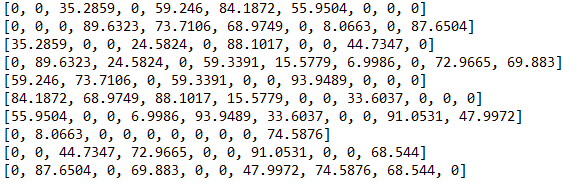
\includegraphics[width=\columnwidth]{assets/graph.png}
    \caption{Example graph of ten vertices utilizing random node deletion in an adjacency matrix}
    \label{fig:example_graph}
\end{figure}

The traveling salesman problem is an NP-Hard problem. Exact solutions to the
problem are feasible from a variety of proven conventional algorithms. Of
course, a brute force exhaustive search will yield an optimal path for the
traveling salesman, given its time complexity this method will only work on
small graphs. Trying all the permutations would lie in the polynomial factor of
O(n!). Better exact solutions such as Held-Karp, branch and bound,
cutting-plane, and dynamic programming often yield a slightly better result with
a solution to the problem in time O(n\textsuperscript{n}). In worse case
scenarios depending on the graph environment, these solutions are no better than
an exhaustive search. We have included an exhaustive search and an
implementation of the branch and bound algorithm to compete with our proposed
approach at an optimal solution to the traveling salesman problem that can be
seen in our results and analysis section. Because the genetic hill climber is a
heuristic solution, it is only possible to provide an approximate solution.
These suboptimal algorithms deliver approximated solutions in a reasonable time
greatly reduced from O(n!) or even eclipsing the time of established exact
algorithms O(n\textsuperscript{n}) time. We believe that this type of approach
is appropriate once the graph sizes enlarge to a point where the earlier
mentioned exact solutions would be rendered useless.

\section{Solution}


\section{Perfromance Evaulation}
Firstly, before analysis of our developed genetic hill climber, the results of
the conventional approaches to the traveling salesman problem should be looked
at first. Using our graph environments that were created and discussed earlier
in the problem definition section, we are unable to obtain optimal solutions to
the graphs once the number of nodes passed 15. Graphs of size 20 vertices and
higher, no optimal solutions were able to be found. This could be attributed to
the circumstances of our testing machine. In attempts to find the optimal
solution either using an exhaustive search or the branch and bound algorithm,
our machine ran for several hours until an abort was conducted due to a
limitation of memory. For the graph of 15 nodes, utilizing an exhaustive search,
the solution was found after a surplus of many hours though the exact runtime
was not recorded. For the branch and bound algorithm running on a graph of 15
nodes, the run time was a $339.85$ seconds. Additionally, it must be pointed out
that the solutions that were obtained via branch and bound were not as optimal
and exact in comparison to the exhaustive search. Our accuracy metric for
evaluating these solutions uses a fitness definition that can be defined as the
total amount of length found in the circuit divided by the total amount of
nodes. This could possibly be due to our implementation of the branch of bound
algorithm where certain branches are excluded from the optimal solution due to
the graphs not being complete. These dead ends in the graph could result in the
algorithm failing to find the global maximum. This can be seen where only the
optimal fitness is equal for the graph of five nodes. Once the graph increases
to a size of ten and 15 nodes, the fitness differs between the branch and bound
algorithm compared exhaustive search.

These results show that these traditional solutions to the traveling salesman
problem are not reliable once a graph scales to a certain size. It is very easy
for real world applications to require more than 15 nodes. Once again it must be
emphasized that in this situation the limiting factor would be our machine when
conducting these tests. This data and conclusion can be drawn once referencing
table \ref{table:branch_and_bound_table}, where there are blanks in columns one
through five from a lack of data that could not be obtained for graphs of nodes
greater than 15. Attempting to fit the branch and bound algorithm on a time
complexity chart shows poorly with our test data of three points. As can be
seen in figure \ref{fig:branch_and_bound_time_complexity}, due to scaling, even
if a fourth point were to be obtained with an X-axis of 20 nodes, the line of
best fit for a graph of n\textsuperscript{n} would project to be a near vertical
line.

\begin{table}[h]
    \setlength\tabcolsep{2pt}
    \centering
    \begin{tabular}{c|c|c|c|c}
    \multicolumn{5}{c}{\textbf{Branch and Bound}}                                                   \\
    \hline
    \text{Nodes} & \text{Time(seconds)} & \text{Fitness} & \text{Optimal Fitness} & \text{\% Error} \\
    \hline
    5            & $0.0004961$          & $74.08426$     & $74.08426$             & $0$             \\
    10           & $0.0168638$          & $57.99643$     & $45.86036$             & $0.26463$       \\
    15           & $339.8524076$        & $50.03704$     & $18.30926$             & $1.73288$       \\
    20           & -                    & -              & -                      & -               \\
    25           & -                    & -              & -                      & -               \\
    50           & -                    & -              & -                      & -               \\
    75           & -                    & -              & -                      & -               \\
    100          & -                    & -              & -                      & -               \\
    125          & -                    & -              & -                      & -               \\
    150          & -                    & -              & -                      & -               \\
    175          & -                    & -              & -                      & -               \\
    200          & -                    & -              & -                      & -               \\
    300          & -                    & -              & -                      & -               \\
    400          & -                    & -              & -                      & -               \\
    500          & -                    & -              & -                      & -               \\
\end{tabular}


    \caption{Runtimes and fitness of the Branch and Bound algorith in comparison to the optimal fitness found in an exhaustive search}
    \label{table:branch_and_bound_table}
\end{table}

\begin{figure}[h]
    \centering
    \textbf{Branch and Bound Time Complexity}
    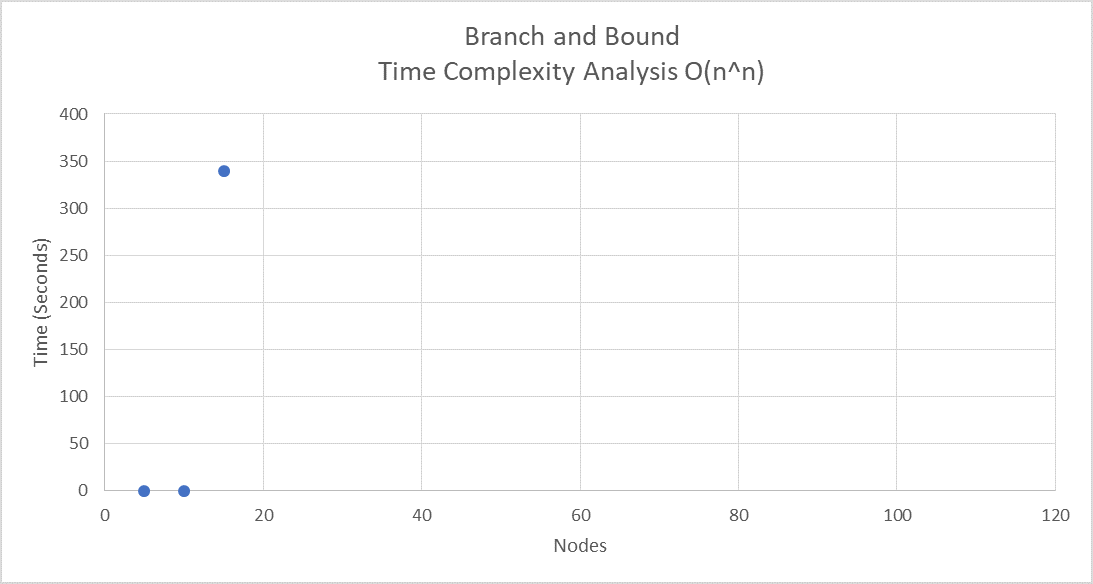
\includegraphics[width=\columnwidth]{assets/branch_and_bound_time_complexity.png}
    \caption{Time complexity of the Branch and Bound algorithm using limited runtime data}
    \label{fig:branch_and_bound_time_complexity}
\end{figure}

Next, upon examination, our stochastic hill climber, which eventually will be
developed as a genetic hill climber, provided us with appalling results. The
stochastic hill climber was able to quickly traverse the graphs and provide
solutions where the other conventional methods were not. At one end of the
spectrum with a graph of five vertices, it was able to obtain the same optimal
fitness as both the branch and bound algorithm as well as the exhaustive search
with a fitness of $74.08426$. Although this is not much of an achievement given
the small size of the graph. The run times were comparable as well within ten
thousandths of a second. These times were kept until a graph of 50 nodes was
introduced where the hill climber took a thousandth of a second to calculate a
heuristic solution. These quick times continued all the way to the other end of
the spectrum with a $0.28519$ second run time for a graph of 500 nodes. These
data values can be seen in table \ref{table:hill_climber_table}. As
mathematically defined in the solutions section, this a glaring obvious
difference between a time complexity of O(n\textsuperscript{n}) and a time
complexity of O(n\textsuperscript{2}).  The stochastic hill climber time
complexity chart can be seen in figure \ref{fig:hill_climber}. Despite these
quick times, due to our limitations of the other conventional approach, we are
unsure of how our fitness that was obtained from the stochastic hill climber
compares to an optimal fitness. In other words, even though a solution was
generated, we are unsure of how accurate and optimal this solution is. This just
goes to show the complexity of the NP-Hard problem that is the traveling
salesman.

\begin{table}[h]
    \setlength\tabcolsep{2pt}
    \centering
    \begin{tabular}{c|c|c|c|c}
    \multicolumn{5}{c}{\textbf{Stochastic Hill Climber}}                                            \\
    \hline
    \text{Nodes} & \text{Time(seconds)} & \text{Fitness} & \text{Optimal Fitness} & \text{\% Error} \\
    \hline
    5            & $0.0004804$          & $74.08426$     & $74.08426$             & $0$             \\
    10           & $0.0004966$          & $55.173$       & $45.86036$             & $0.20299$       \\
    15           & $0.0004954$          & $28.21844$     & $18.30926$             & $0.54121$       \\
    20           & $0.0009851$          & $21.96413$     & -                      & -               \\
    25           & $0.0004961$          & $23.15343$     & -                      & -               \\
    50           & $0.0014879$          & $18.45314$     & -                      & -               \\
    75           & $0.0034711$          & $13.36534$     & -                      & -               \\
    100          & $0.0064475$          & $13.24880$     & -                      & -               \\
    125          & $0.0089280$          & $14.08632$     & -                      & -               \\
    150          & $0.0143837$          & $11.71591$     & -                      & -               \\
    175          & $0.0183513$          & $9.423754$     & -                      & -               \\
    200          & $0.0247995$          & $11.53126$     & -                      & -               \\
    300          & $0.0709278$          & $12.72170$     & -                      & -               \\
    400          & $0.1547515$          & $7.936304$     & -                      & -               \\
    500          & $0.2851998$          & $9.040675$     & -                      & -               \\
\end{tabular}
    \caption{Run times of the Stochastic Hill-Climber and obtained Fitness}
    \label{table:hill_climber_table}
\end{table}

\begin{figure}[h]
    \centering
    \textbf{Stochastic Hill Climber Time Complexity}
    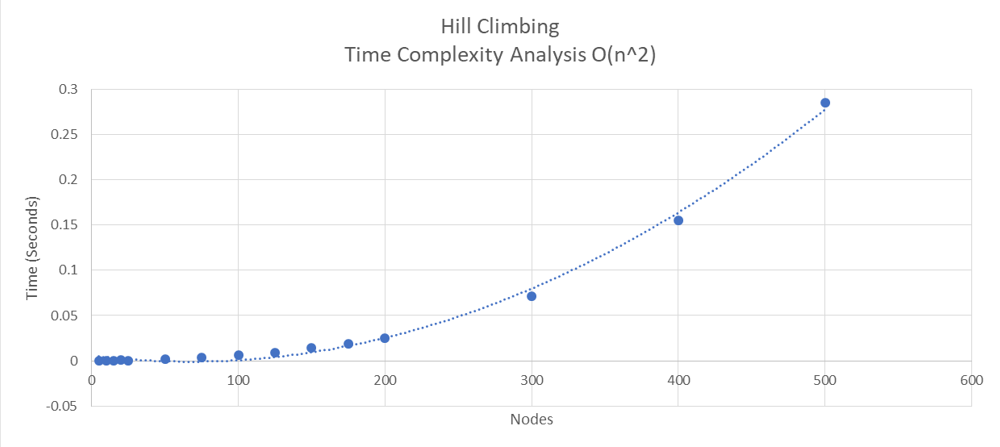
\includegraphics[width=\columnwidth]{assets/hill_climber.png}
    \caption{asdf}
    \label{fig:hill_climber}
\end{figure}

asdf
asdfasdf
asdf
asdfasdf
asdfasdf
asdfasdf
asdfasdfasdf
asdfasdf
asdf
asdfasdf
asdfasdf
asdfasdf
asdfasdfasdf
asdfasdf
asdf
asdfasdf
asdfasdf
asdfasdf
asdfasdfasdf
asdfasdf
asdf
asdfasdf
asdfasdf
asdfasdf
asdfasdfasdf
asdfasdf
asdf
asdfasdf
asdfasdf
asdfasdf
asdfasdf

asdf
asdfasdf
asdf
asdfasdf
asdfasdf
asdfasdf
asdfasdfasdf
asdfasdf
asdf
asdfasdf
asdfasdf
asdfasdf
asdfasdfasdf
asdfasdf
asdf
asdfasdf
asdfasdf
asdfasdf
asdfasdf
asdf
asdfasdf
asdf
asdfasdf
asdfasdf
asdfasdf
asdfasdf

asdf
asdfasdf
asdf
asdfasdf
asdfasdf
asdfasdf
asdfasdfasdf
asdfasdf
asdf
asdfasdf
asdfasdf
asdfasdf
asdfasdfasdf
asdfasdf
asdf
asdfasdf
asdfasdf
asdfasdf
asdfasdfasdf
asdfasdf
asdf
asdfasdf
asdfasdf
asdfasdf
asdfasdfasdf
asdfasdf
asdf
asdfasdf
asdfasdf
asdfasdf
asdfasdf

asdf
asdfasdf
asdf
asdfasdf
asdfasdf
asdfasdf
asdfasdfasdf
asdfasdf
asdf
asdfasdf
asdfasdf
asdfasdf
asdfasdfasdf
asdfasdf
asdf
asdfasdf
asdfasdf
asdfasdf
asdfasdf
asdf
asdfasdf
asdf
asdfasdf
asdfasdf
asdfasdf
asdfasdf


\section{Prognosis}

\section{Conclusion and Future Work}


\bibliographystyle{ACM-Reference-Format}
\bibliography{report}

\end{document}
\endinput
